\documentclass[frenchb,11pt]{article}
\usepackage[T1]{fontenc}
\usepackage[utf8]{inputenc}
\usepackage{a4, fullpage, times}
\usepackage{graphicx, amsmath, moreverb}
\usepackage{amssymb} 

\usepackage{babel}
\makeatother
\begin{document}

\noindent
{\bf Université de Strasbourg}
\hfill
{\bf UFR Mathématique et Informatique}

\vskip 0.5 cm

\begin{center}
{\huge Le tour de magie}
\end{center}

\hspace*{-\parindent}%
\begin{minipage}{0.60\linewidth}
Le chercheur qui était en face de vous a-t-il découvert l'emplacement du trésor grâce à la magie ?
Dans les fait, non, il a simplement utilisé ce qu'on appelle un code correcteur / détecteur d'erreurs.
De tels codes sont utilisés régulièrement dans différents domaines afin de détecter (on sait qu'il y a une erreur mais la position de cette erreur n'est pas identifiable) ou corriger des erreurs (la position de l'erreur est connue et on peut par conséquent la corriger).
Par exemple, les numéros de compte bancaire ou les numéros de sécurité sociale utilisent des codes détecteurs d'erreurs.
Ils sont également massivement utilisés en informatique dans les supports numériques (disque dur, CD, Blu-ray), les communications réseaux, etc.
\end{minipage}
\begin{minipage}{0.05\linewidth}
\hfill
\end{minipage}
\begin{minipage}{0.35\linewidth}
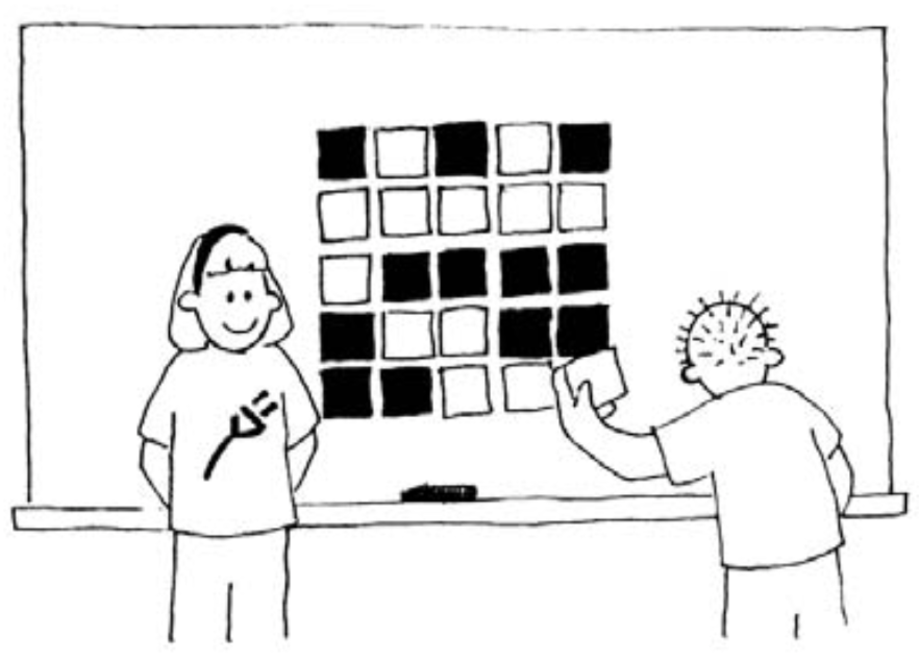
\includegraphics[width=0.95\textwidth]{intro.pdf}
\end{minipage}

\vskip 0.1cm
\noindent
Le code correcteur d'erreurs utilisé dans le tour qui vous a été présenté est appelé \textit{code à parité horizontale et verticale}.
Il permet de détecter deux erreurs ou d'en corriger une.
Pour ce faire, l'idée est d'ajouter une case supplémentaire à chaque ligne et colonne de sorte que chaque ligne ou colonne comporte un nombre pair de jeton vert.
Dans la suite nous détaillons le fonctionnement de ce code.

\section*{La parité}

\noindent
En mathématique, la parité est la propriété d'un entier à se classer dans l'une des deux catégories : pair ou impair.
Un entier est pair s'il est divisible par 2 (le reste de la division entière par 2 est nul).
Dans le cas contraire il est impair.
Par exemple le nombre 6 est pair ($6/3 = 2$) alors que 7 est impair ($7/2 = 3$ reste $1$).

\section*{Code à parité horizontale}

\hspace*{-\parindent}%
\begin{minipage}{0.6\linewidth}
Pour illustrer le code détecteur d'erreurs à parité horizontale on considère un tableau composé de 1 ligne et de 5 colonnes dans lequel chaque case peut prendre la couleur noire ou blanche.
Supposons qu'on dispose de 3 cases noires et de 2 cases blanches.
Pour pouvoir détecter qu'une case a changé de couleur (et donc une erreur), la phase de codage nécessite d'ajouter une case supplémentaire.
Par construction, on choisit que le nombre de cases noires de l'ensemble doit être un nombre pair (le choix de la couleur importe peu mais il faut en choisir une).
Dans notre exemple il faut par conséquent que la 6e case soit noire pour avoir un total de 4 cases noires comme illustré sur la figure ci-contre.
\end{minipage}
\begin{minipage}{0.4\linewidth}
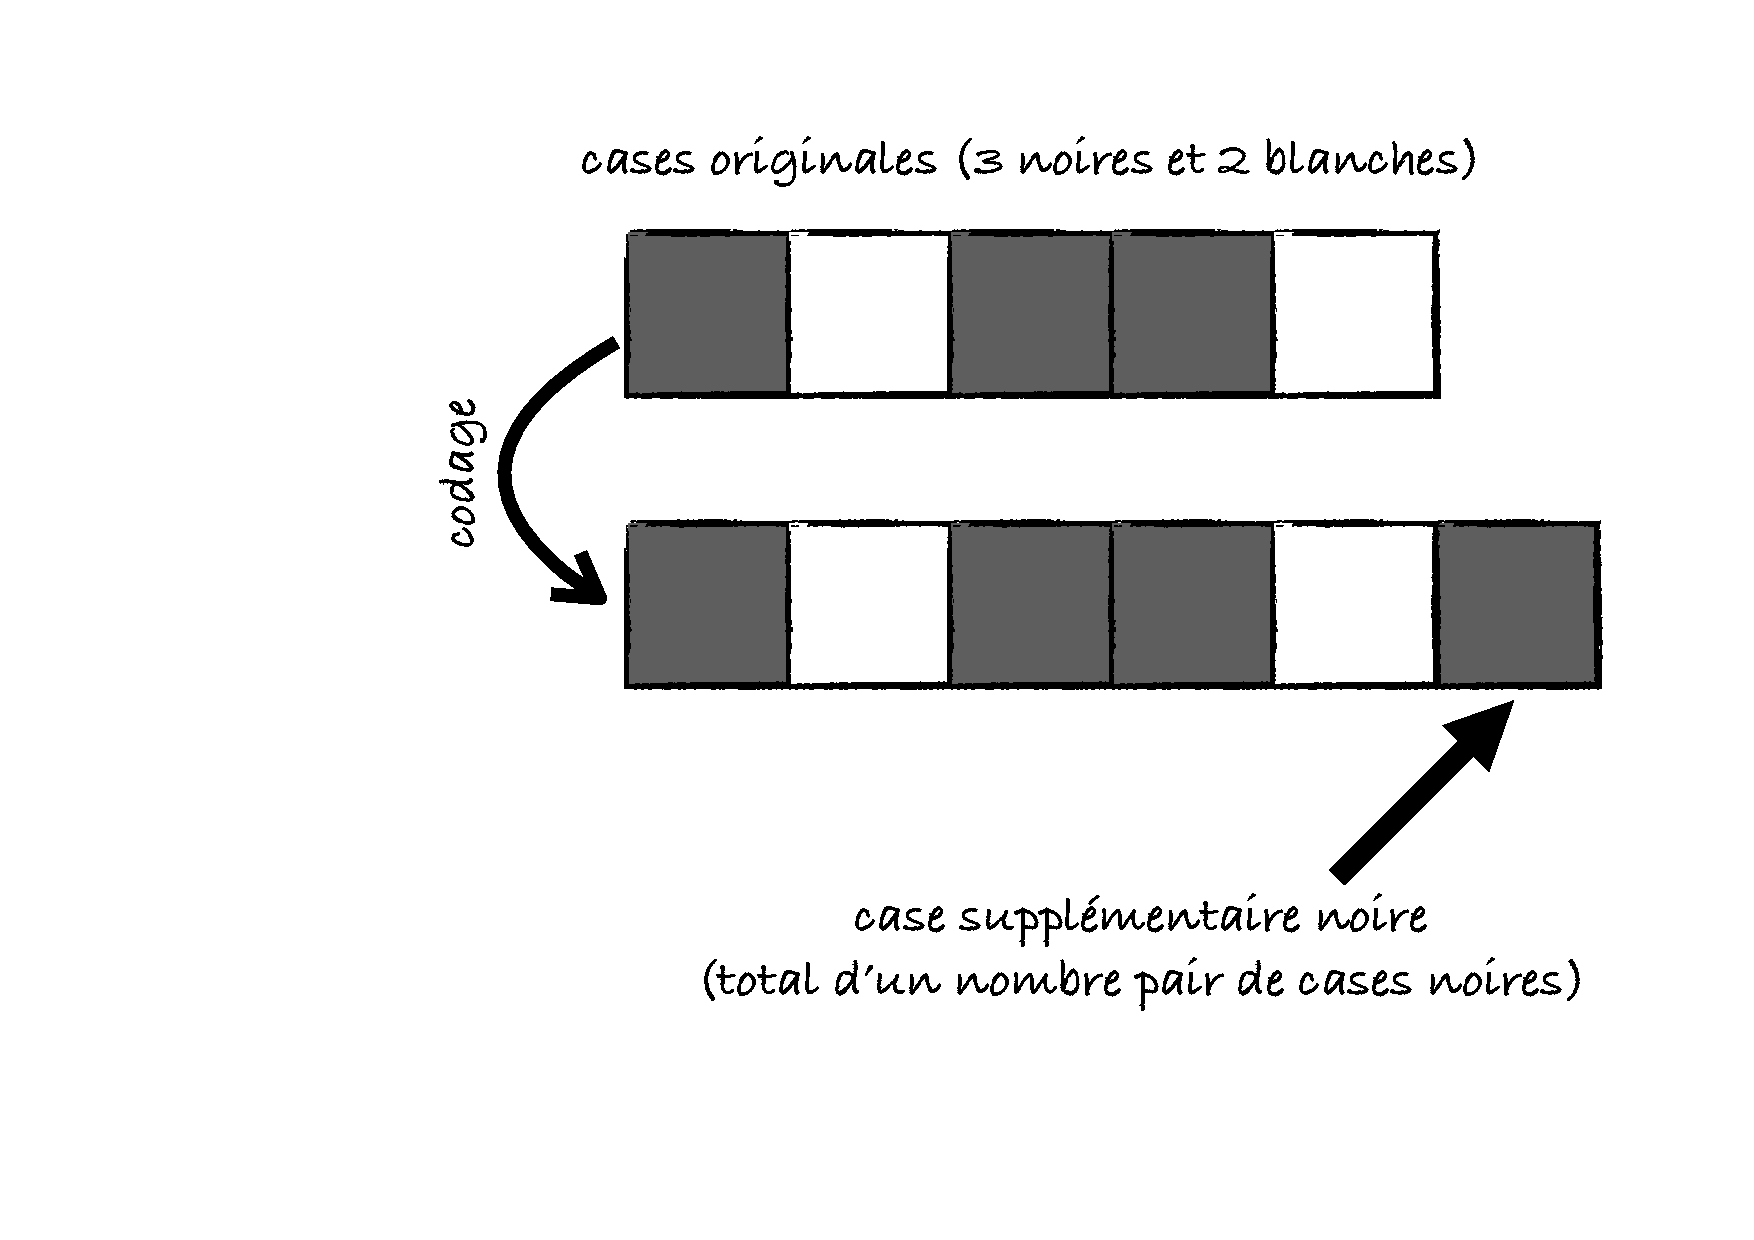
\includegraphics[width=0.99\textwidth]{building.pdf}
\end{minipage}

\begin{minipage}{0.40\linewidth}
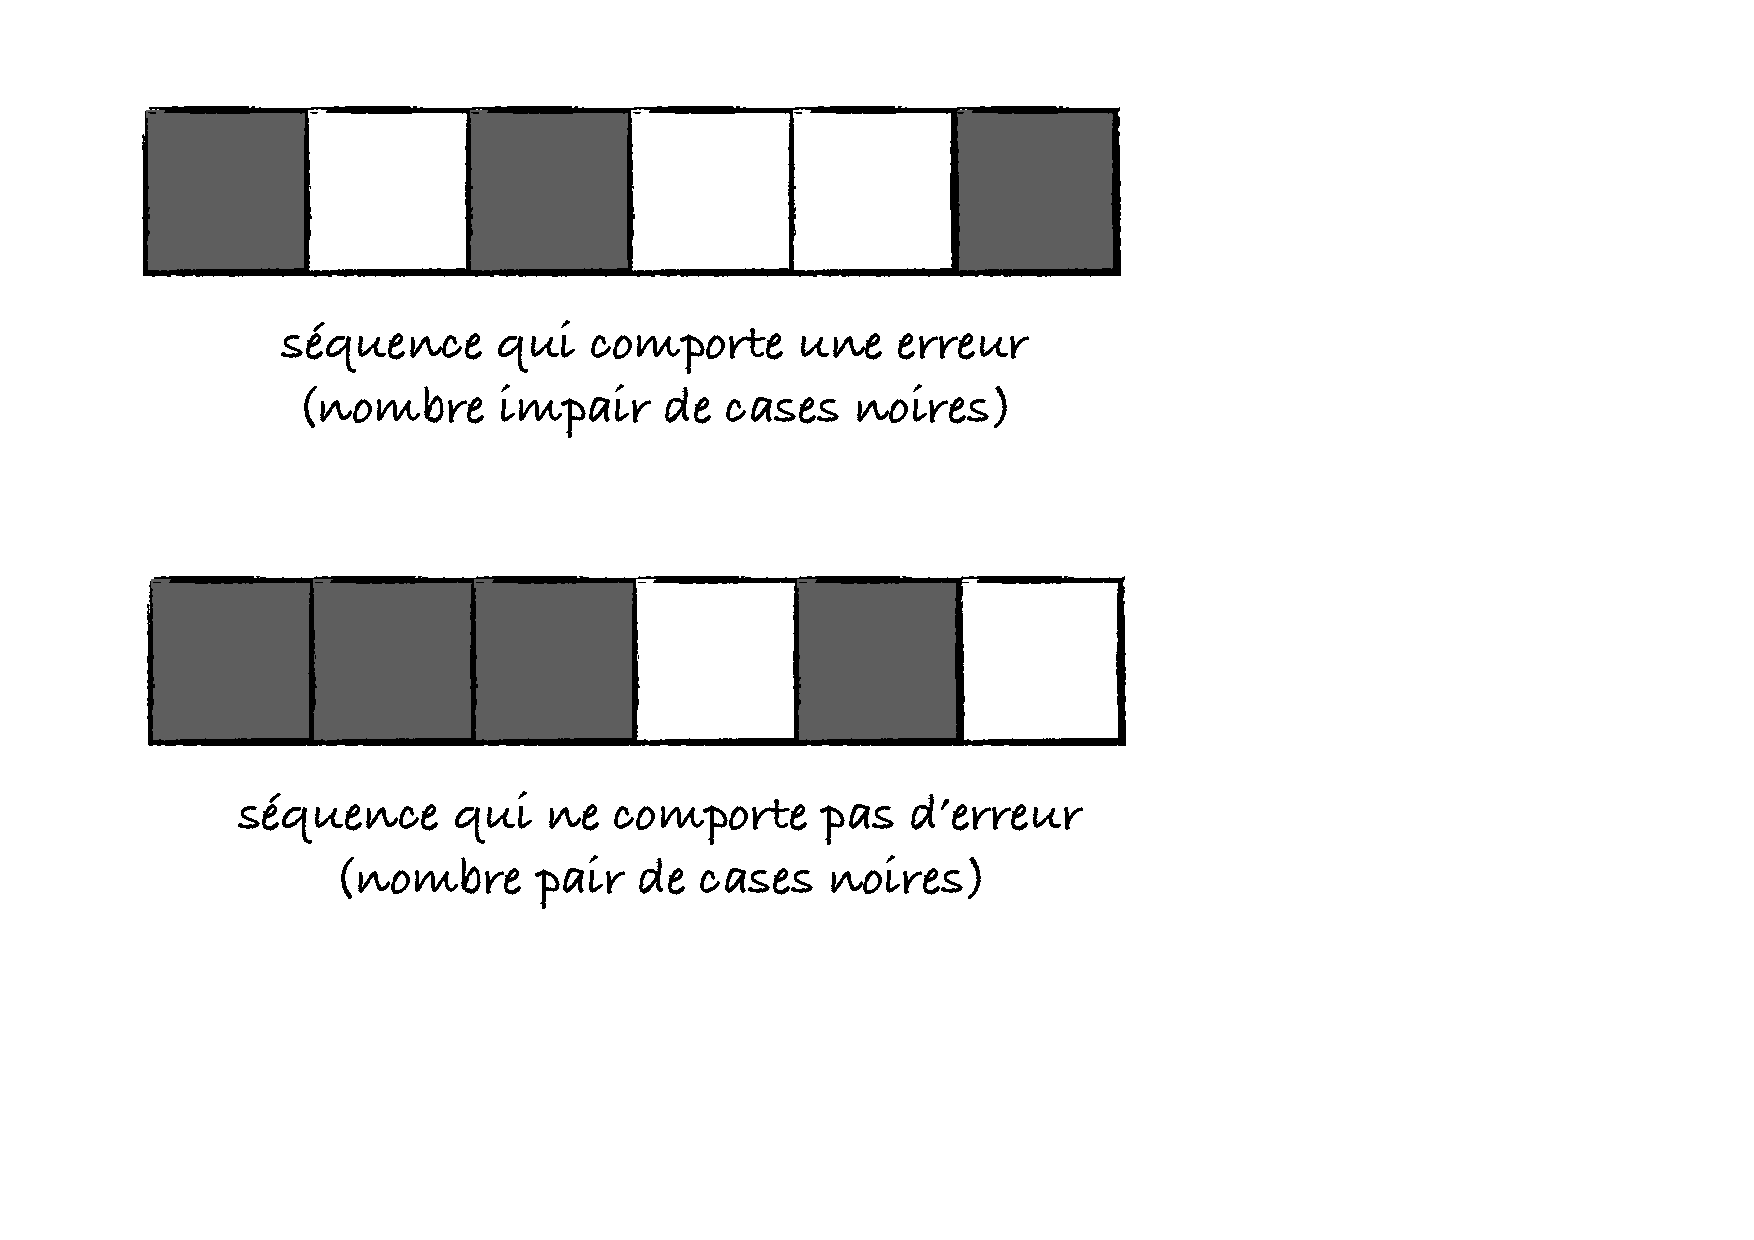
\includegraphics[width=0.95\textwidth]{error-seq.pdf}
\end{minipage}
\begin{minipage}{0.55\linewidth}
Au décodage, si au plus une erreur est présente, cela signifie qu'une case noire est devenue blanche ou inversement.
Quelle que soit la position de ce changement et donc de cette erreur, le nombre total de cases noires ne sera plus pair et il devient possible de détecter l'erreur.
Il n'est pas contre pas possible de la corriger car rien ne permet d'identifier le numéro de la case qui a été modifiée.
De plus, si deux erreurs sont présentes sur des cases distinctes, le code à parité horizontale ne permettra pas de les détecter.
Par conséquent, le code à parité horizontale permet de détecter une erreur unique.
D'autres codes disposant d'un pouvoir supérieur de détection / correction existent, notamment le code à parité horizontale et verticale utilisé dans le tour qui vous a été présenté.
\end{minipage}

\section*{Code à parité horizontale et verticale}

L'idée du code à parité horizontale et verticale consiste à appliquer un code à parité horizontale sur chaque ligne, mais également sur chaque colonne.
Après codage, le nombre de cases noires sur chaque ligne et chaque colonne sera pair, comme illustré sur la figure ci-dessous.

\begin{center}
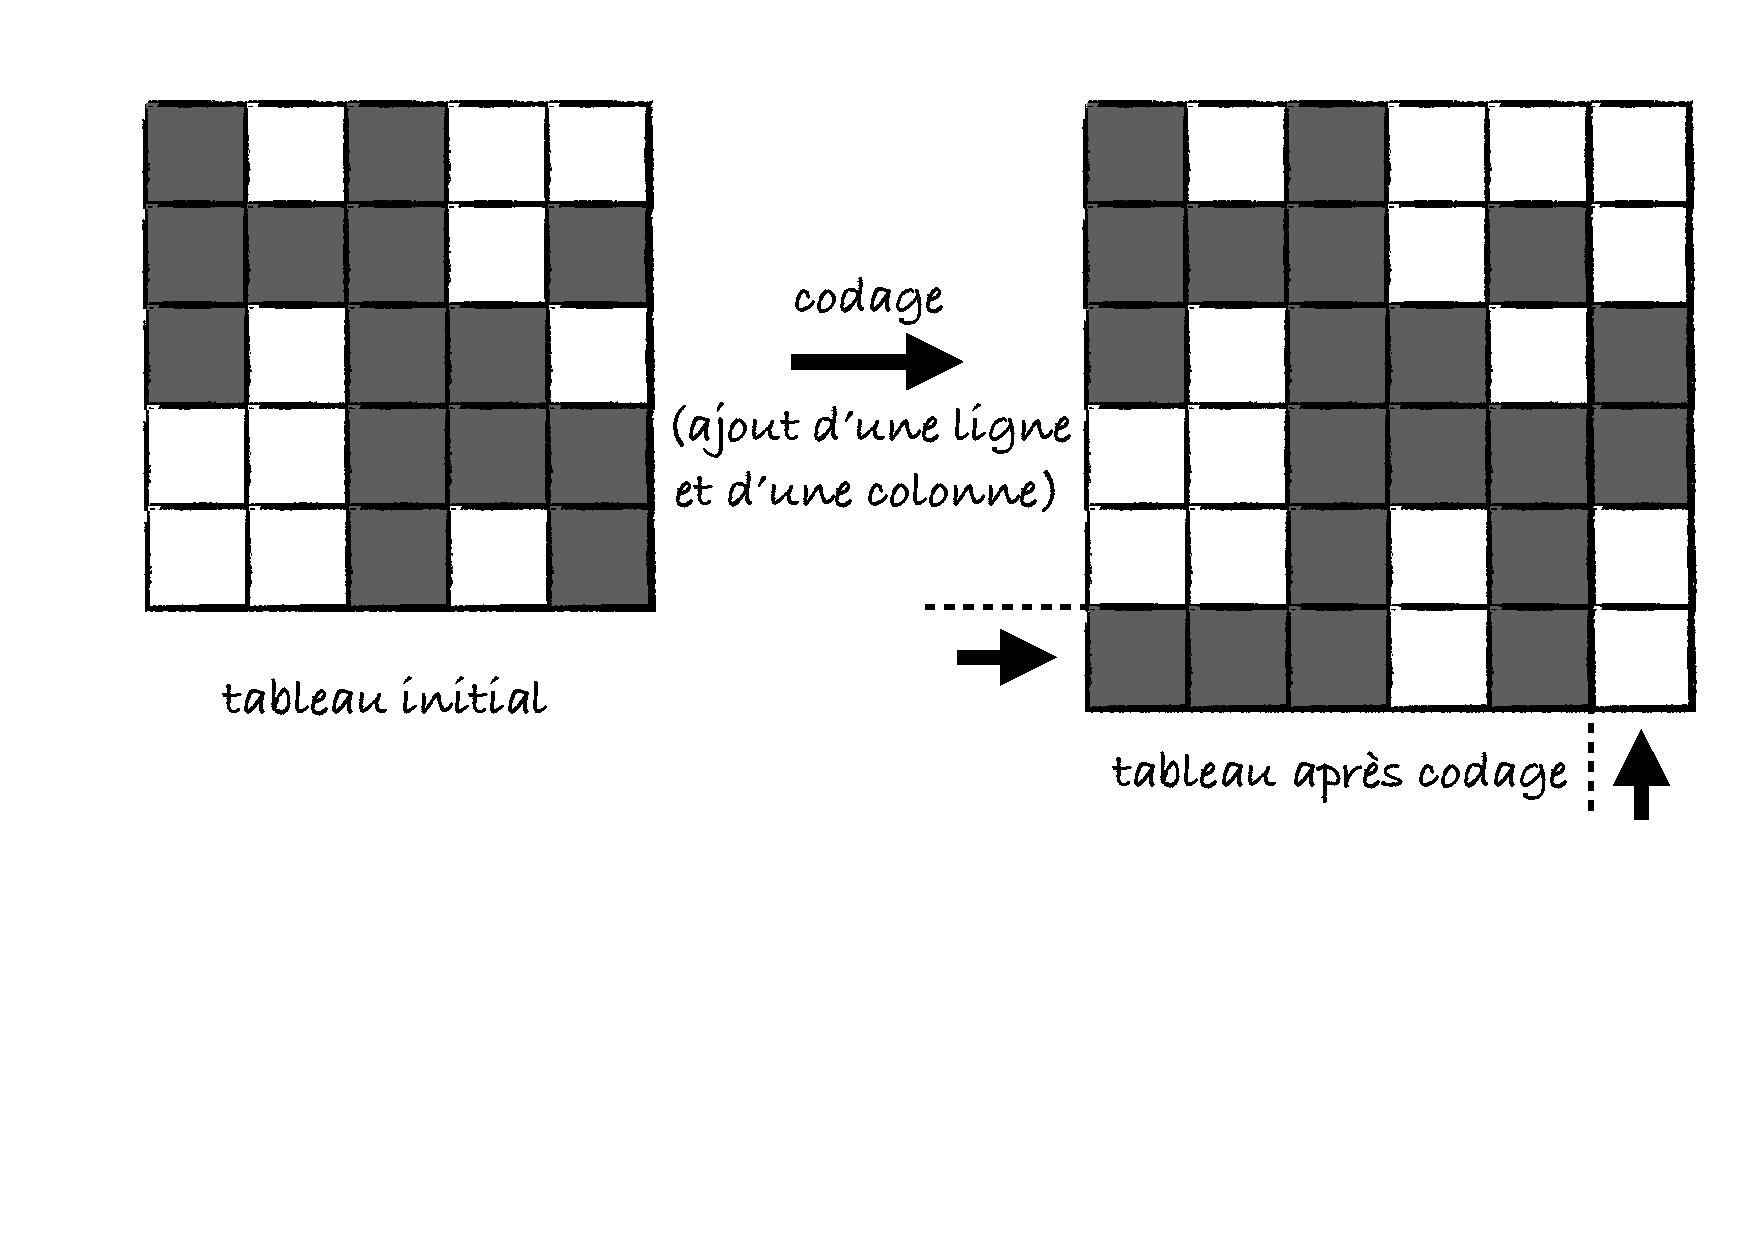
\includegraphics[width=0.70\textwidth]{hv-parity.pdf}
\end{center}

\vskip 0.1cm

\hspace*{-\parindent}%
\begin{minipage}{0.60\linewidth}
Au décodage, si une erreur est présente, la ligne et la colonne dont le nombre de cases noires n'est pas pair permettent d'identifier la case qui comporte une erreur.
Sur l'exemple ci-contre, on voit que la 3e ligne et que la 3e colonne comportent chacune un nombre impair de cases noires.
Cela implique que la case qui appartient à cette ligne et à cette colonne comporte une erreur (la case devrait être noire et non blanche).
C'est par ce moyen que le chercheur a réussi à trouver où se cachait le trésor.
Le code à parité horizontale et verticale permet de corriger une erreur ou de détecter jusqu'à deux erreurs.
D'autres codes disposant d'un plus grand pouvoir de détection / correction existent, tels que les codes de Hamming ou Reed-Solomon, mais ils sont plus complexes à mettre en \oe{}uvre.
\end{minipage}
\begin{minipage}{0.4\linewidth}
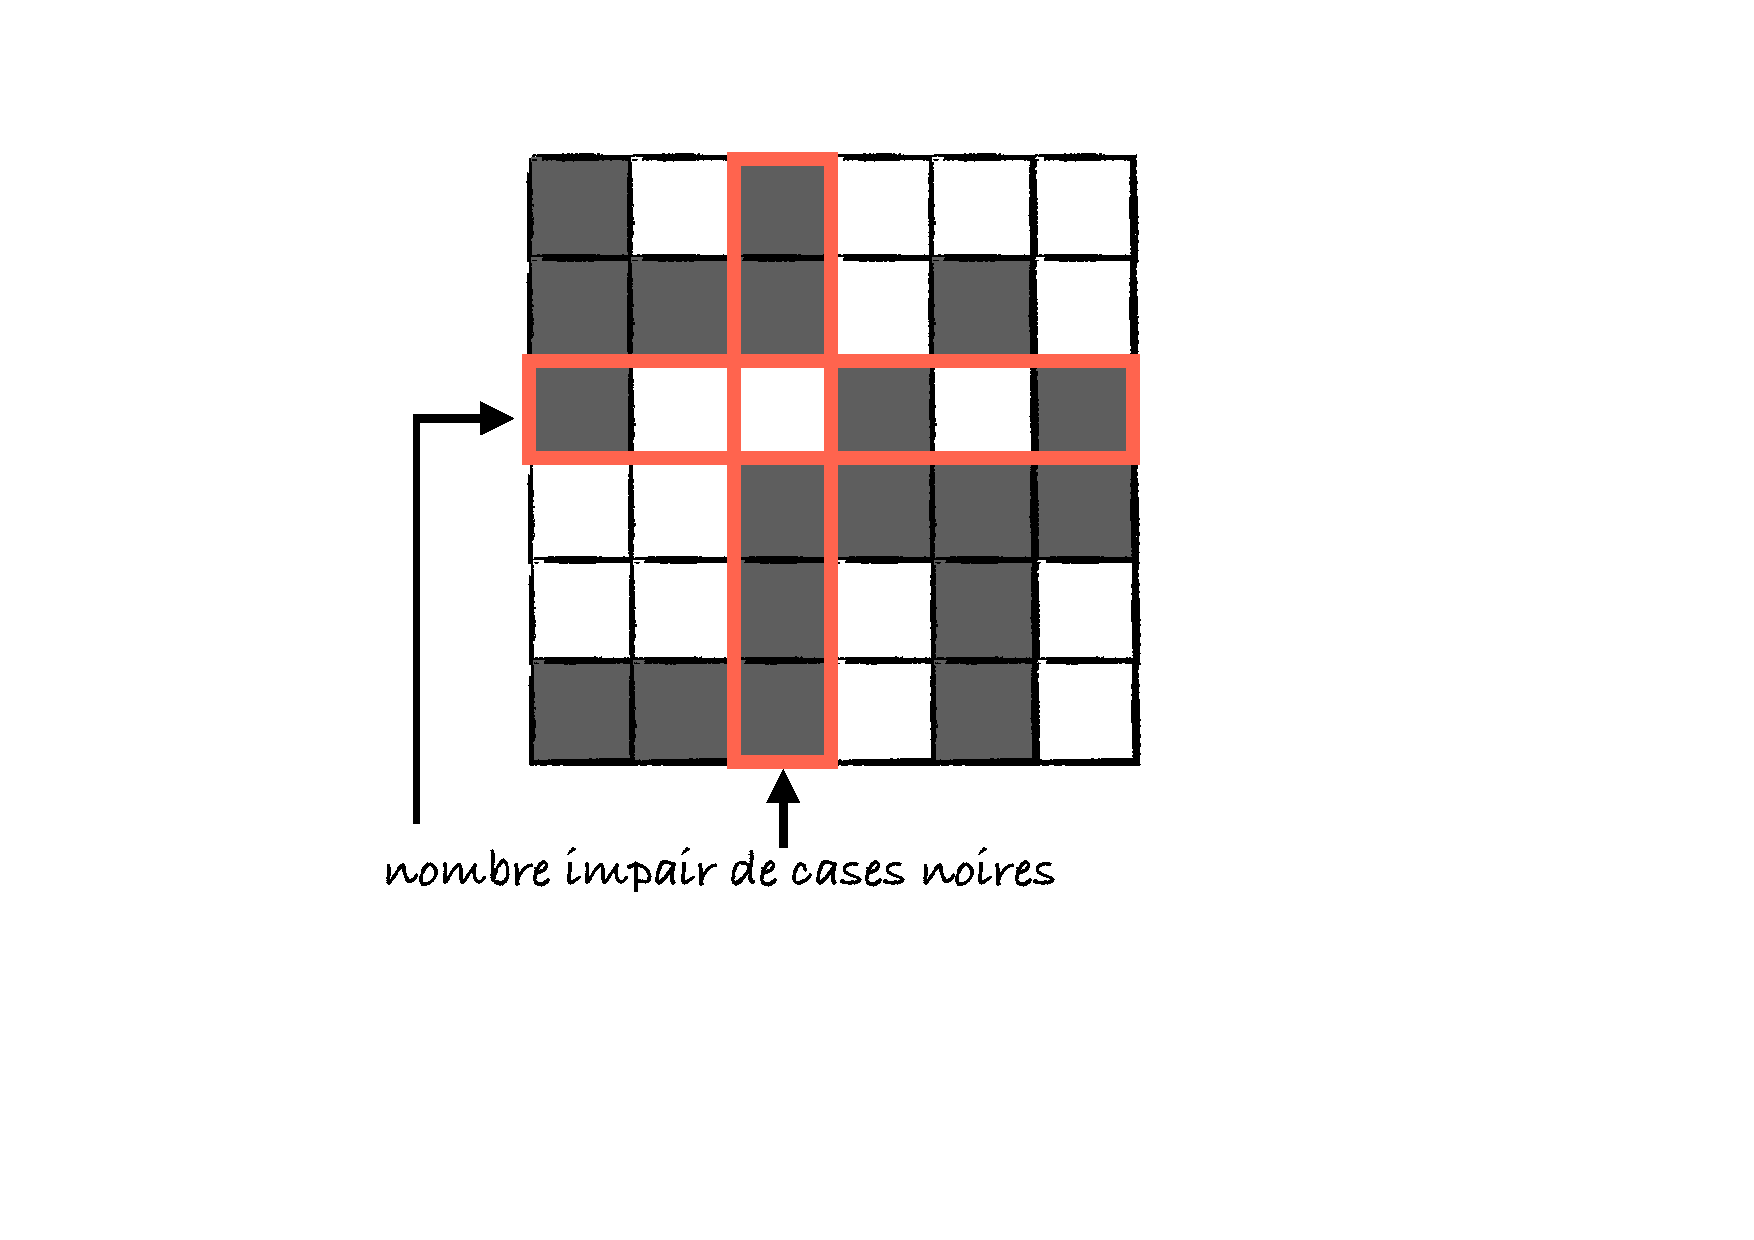
\includegraphics[width=0.95\textwidth]{hv-error.pdf}
\end{minipage}

%\section*{Pour aller plus loin}

\end{document}
